
%(BEGIN_QUESTION)
% Copyright 2015, Tony R. Kuphaldt, released under the Creative Commons Attribution License (v 1.0)
% This means you may do almost anything with this work of mine, so long as you give me proper credit

The {\it R-value} of an insulating material is defined as the quotient of length ($l$) and thermal conductivity ($k$), both from the heat conduction equation:

$$R = {l \over k}$$

$${dQ \over dt} = {kA {\Delta T} \over l}$$

Modify the heat conduction equation to incorporate $R$ instead of $k$, and then use it to calculate the heat loss rate through the surfaces of the following box, insulated with R-30 insulation ($R$ = 30 ft$^{2}$ $\cdot$ h $\cdot$ F$^{o}$ / Btu), heated internally to a temperature of 75$^{o}$ F, and exposed to an outside (ambient) temperature of 40$^{o}$ F:

$$\includegraphics[width=15.5cm]{i00333x01.eps}$$

Challenge question: if the box is heated solely by an electric light bulb, how large would this light bulb have to be (i.e. its wattage rating) in order to maintain an internal box temperature of 75$^{o}$ F given an outside temperature of 40$^{o}$ F?

\vskip 20pt \vbox{\hrule \hbox{\strut \vrule{} {\bf Suggestions for Socratic discussion} \vrule} \hrule}

\begin{itemize}
\item{} Describe the relationship between insulation R-value and energy efficiency for a heated building. 
\item{} Describe the relationship between insulation R-value and energy efficiency for a cooled (air-conditioned) building. 
\item{} Suppose this box were heated by an electric heating element with an on/off thermostat control to maintain air temperature at or near 75 degrees F.  How would the {\it duty} cycle of this heater (it's on-time divided by the on+off time) vary with changes in outside temperature?
\item{} Demonstrate how to {\it estimate} numerical answers for this problem without using a calculator.
\end{itemize}

\underbar{file i00333}
%(END_QUESTION)





%(BEGIN_ANSWER)

Answer to challenge question: the light bulb would have to be 205 watts (two 100-watt bulbs operating together would come close!).

%(END_ANSWER)





%(BEGIN_NOTES)

An easy way to take $k$ and $l$ out of the equation in favor of $R$ is to solve for $l$ in terms of $R$ and $k$ ($l = kR$), then substitute $kR$ into the conduction equation in place of $l$ and cancel the $k$ on the top and bottom of the fraction:

$${dQ \over dt} = {A {\Delta T} \over R}$$

The total area ($A$) of the box is 600 square feet (six sides, each one having a surface area of 100 square feet).  The temperature differential across the walls of the box is 35 degrees (75 $-$ 40).  The R value is given to us as R-30:

$${dQ \over dt} = {(600) (35) \over 30} = 700 \hbox{ BTU/hour}$$

The conversion factor between BTU/h and watts is 745.7 watts = 2544.43 BTU/h.  Therefore:

$$\left({700 \hbox{ BTU/h} \over 1}\right) \left( {745.7 \hbox{ W} \over 2544.43 \hbox{ BTU/h}} \right) = 205.15 \hbox{ W}$$







\vfil \eject

\noindent
{\bf Summary Quiz:}

Suppose a home requires 12,500 BTU per hour of heat input to maintain a room temperature of 70 degrees Fahrenheit on a day when the outside temperature is 30 degrees Fahrenheit.  Calculate the approximate heat input rate required to maintain the same room temperature if the weather warms up to 50 degrees Fahrenheit, assuming all other factors remain the same.

\begin{itemize}
\item{} 3,125 BTU per hour
\vskip 5pt 
\item{} 25,000 BTU per hour 
\vskip 5pt 
\item{} 6,250 BTU per hour
\vskip 5pt 
\item{} 100,000 BTU per hour
\vskip 5pt 
\item{} 12,500 BTU per hour 
\vskip 5pt 
\item{} 50,000 BTU per hour
\end{itemize}

%INDEX% Measurement, heat: conduction through a solid substance

%(END_NOTES)


